\documentclass{beamer}

\usepackage{multicol}
\usepackage{verbatim}
\usepackage{subcaption}

\usetheme{Padova}

\title{Visualizzazione volumetrica 3D di immagini radiologiche}
\subtitle{
Dipartimento di Matematica "Tullio Levi-Civita"
\\
Università degli Studi di Padova
\\
Corso di laurea in Informatica
}
\author{Michele Roverato}
\date{16 dicembre 2020}

\begin{document}

	%-----------------------------------------	

	\maketitle
	
	%-----------------------------------------	
	
	\section{Avviso}
	\begin{frame}{Introduzione}
	
	\begin{alertblock}{Attenzione}
	Questa presentazione includerà immagini radiologiche
	\end{alertblock}
	
	\begin{multicols}{2}
		Cosa vedremo:
		\begin{itemize}
			\item Radiografie;
			\item Ricostruzioni 3D di radiografie.
		\end{itemize}

		\columnbreak

		Cosa non vedremo:
		\begin{itemize}
			\item Sangue;
			\item Foto reali di pazienti o di organi.
		\end{itemize}
	\end{multicols}
	
	\end{frame}
	
	%-----------------------------------------	

	%Comment section just to keep track how to do special blocks
	\begin{comment}

	\begin{frame}{First section}
		\begin{block}{Normal block}
			Fusce luctus venenatis felis quis semper
		\end{block}

		\begin{alertblock}{Alert block}
			$$ E = (x_1 \vee \neg x_2 \vee \neg x_3) \wedge (x_1 \vee x_2 \vee x_4) $$
		\end{alertblock}

		\begin{exampleblock}{Example block}
			Proin tincidunt, neque at tincidunt mollis
		\end{exampleblock}
	\end{frame}
	
	\end{comment}

	%-----------------------------------------	
	
	\section{Azienda}
	\begin{frame}{Azienda} 
	
	\begin{figure}[ht]
    	\centering
    	
\includegraphics[width=0.5\textwidth]{Images/logo-azienda.png}
	\end{figure}	
	
	\begin{itemize}
		\item Nata nel 2008 con sede legale a Vicenza;
		\item Filosofia incentrata su spirito di squadra, rispetto delle regole e valore alla persona e al merito.
	\end{itemize}
	
	Offre:
	\begin{itemize}
		\item Interfacciamento con macchine diagnostiche digitali;
		\item Consulenze per reti di macchine diagnostiche;
		\item Elaborazione di immagini diagnostiche specializzate.
	\end{itemize}
	
	
	\end{frame}
	
	%-----------------------------------------	
	
	\section{Ricerca e discussione stage}
	\begin{frame}{Ricerca e discussione stage}
	
	\begin{figure}[ht]
    	\centering
    	
\includegraphics[width=0.5\textwidth]{Images/stageit2019.png}
	\end{figure}
	
	\begin{itemize}
		\item Partecipazione a StageIT 2019;
		\item Ricerca nei documenti passati;
		\item Contatto e discussione con l'azienda.
	\end{itemize}
	
	L'azienda era interessata a:
	\begin{itemize}
		\item Integrare un visualizzatore volumetrico;
		\item Utilizzare CMake come sistema di sviluppo.
	\end{itemize}
	
	\end{frame}
	
	%-----------------------------------------	
	
	\section{Tecnologie utilizzate}
	\begin{frame}{Tecnologie utilizzate}
	
	\begin{figure}[ht]
    	\centering
    	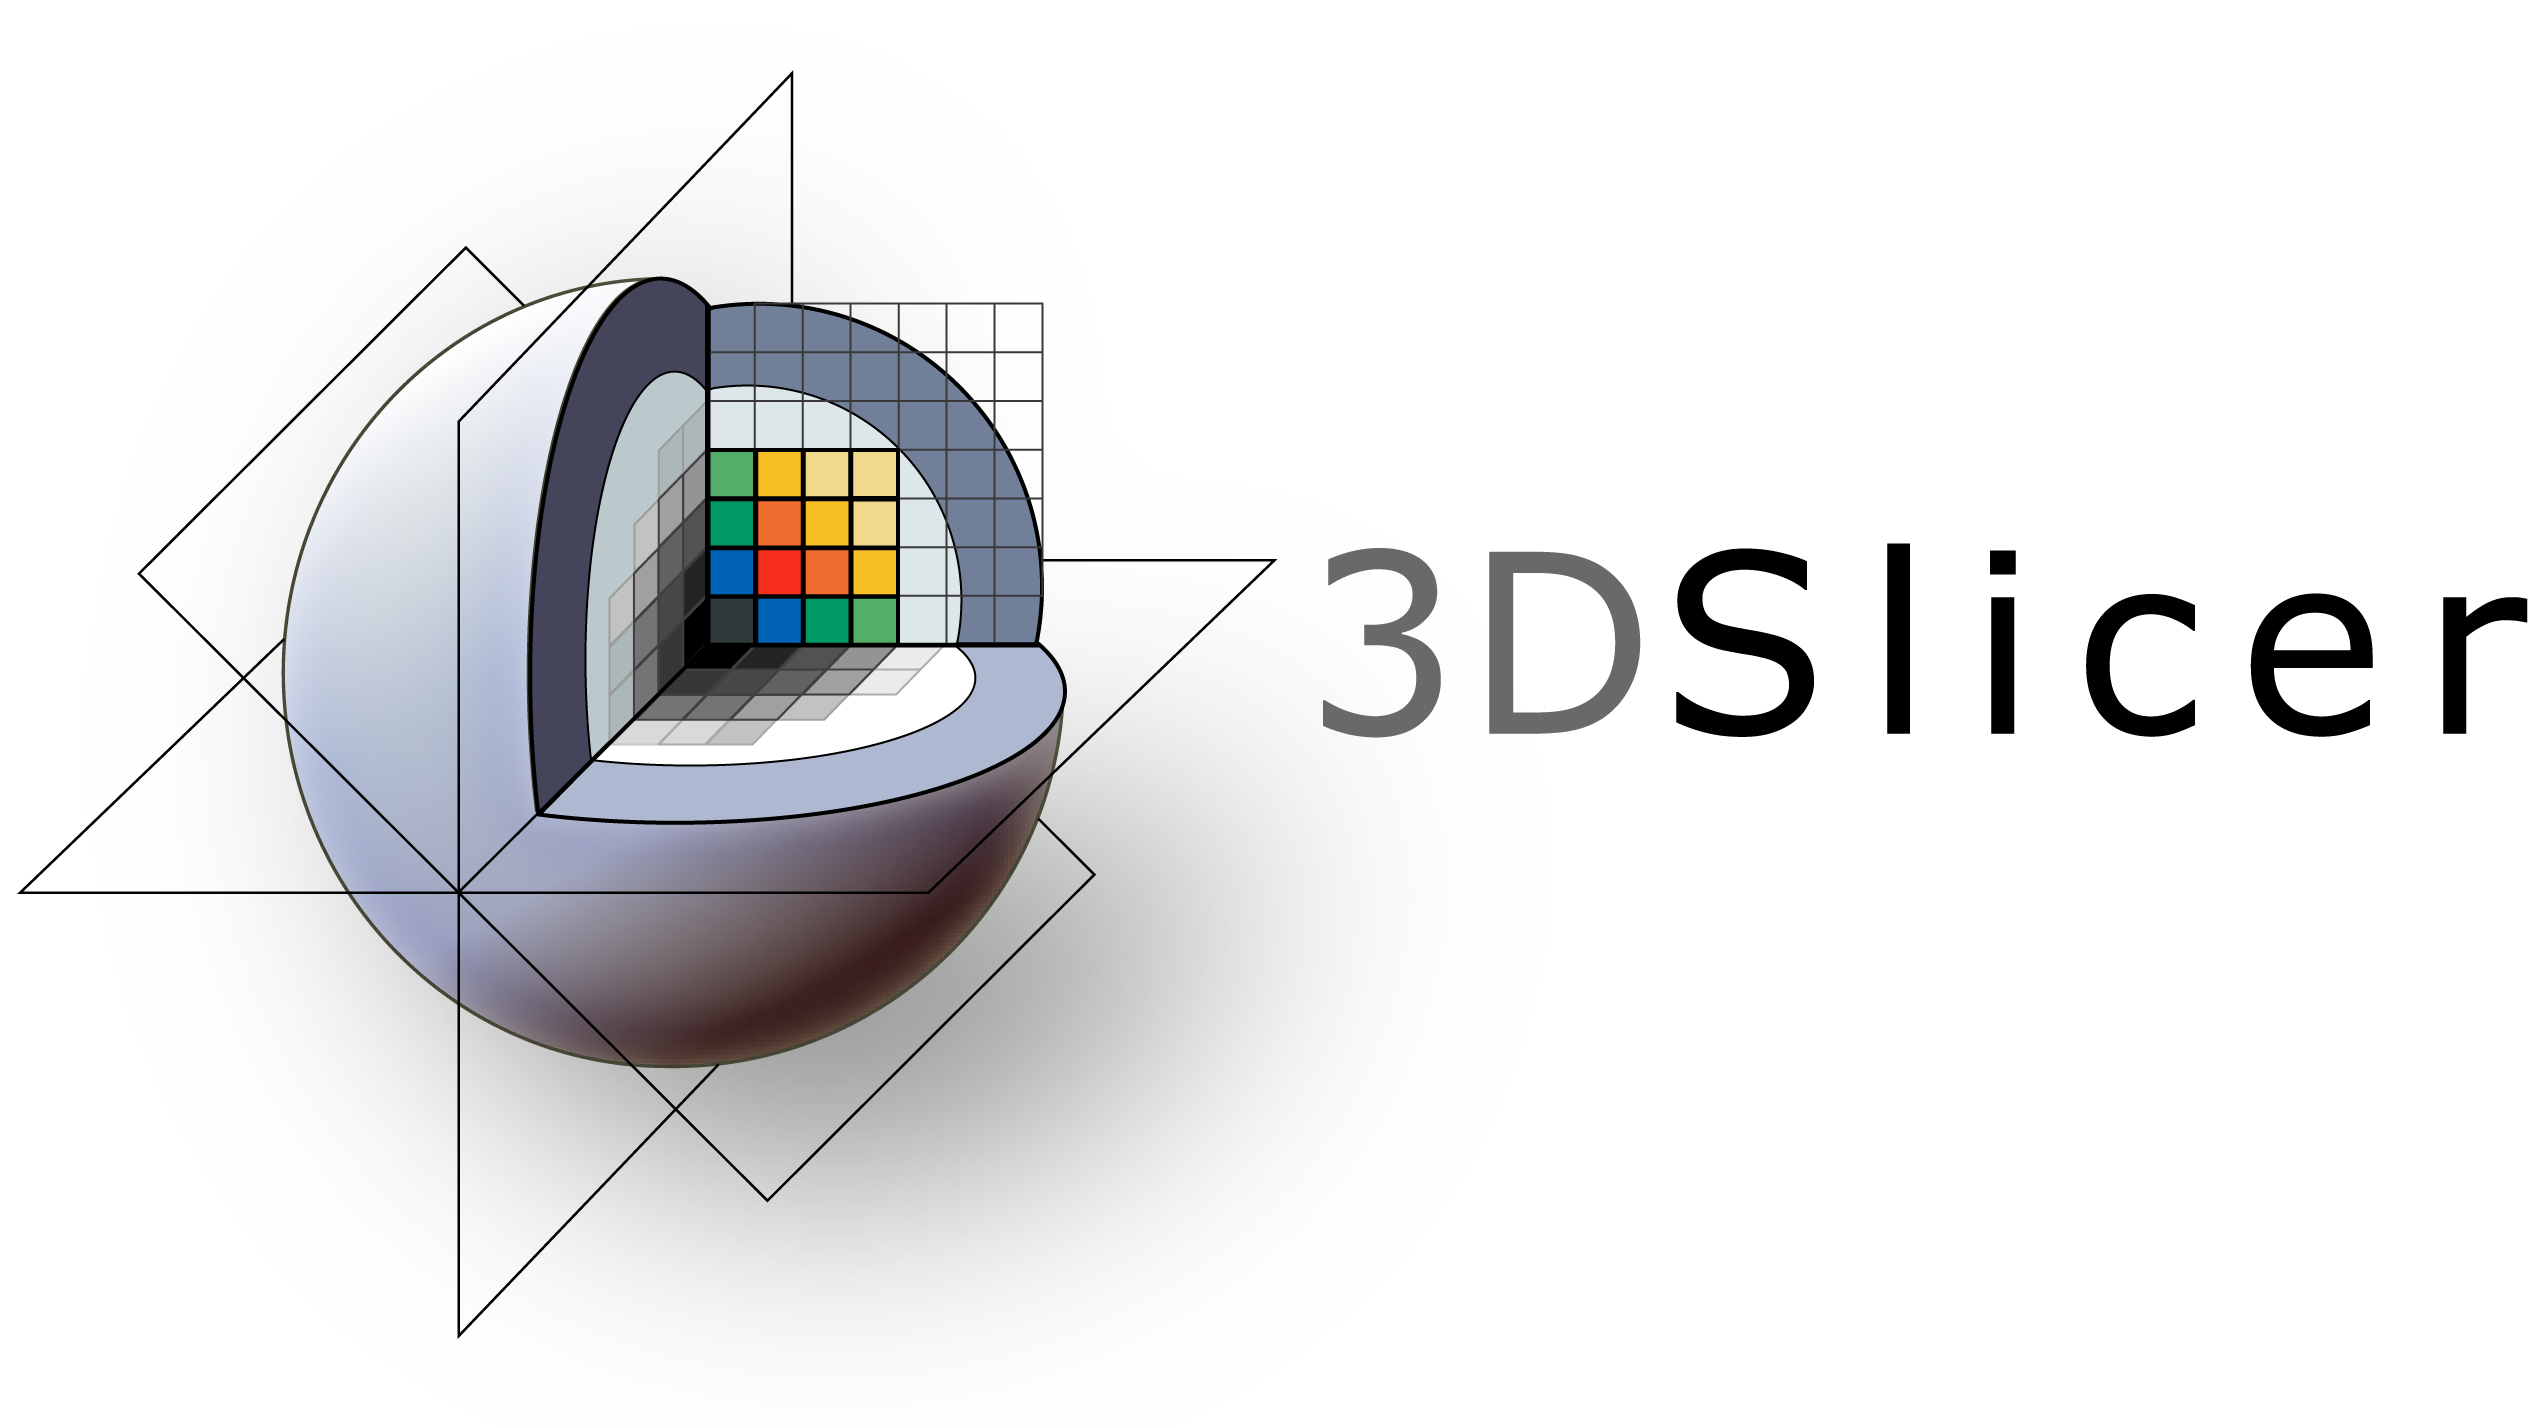
\includegraphics[width=0.3\textwidth]{Images/logo3dslicer.png}
	\end{figure}
	
	\begin{itemize}
		\item Studio di 3D Slicer per comprendere il volume rendering.
	\end{itemize}

	\begin{figure}
		\centering
		\begin{subfigure}{.3\textwidth}
  			\centering
  			
\includegraphics[width=.5\linewidth]{Images/logoqt.png}
		\end{subfigure}
		\begin{subfigure}{.3\textwidth}
  			\centering
  			
\includegraphics[width=1\linewidth]{Images/logocmake.png}
		\end{subfigure}
		\begin{subfigure}{.3\textwidth}
  			\centering
  			
\includegraphics[width=.6\linewidth]{Images/logovtk.png}
		\end{subfigure}
	\end{figure}	
	
	\begin{itemize}
		\item Ripasso concetti di Qt;
		\item Scrittura file di CMake e utilizzo in Visual Studio e Qt Creator;
		\item Studio di VTK.
	\end{itemize}
	
	\end{frame}
	
	%-----------------------------------------	
	
	\section{Rendering Volumetrico}
	\begin{frame}{Rendering Volumetrico}
	
	\begin{figure}
		\centering
		\begin{subfigure}{.4\textwidth}
  			\centering
  			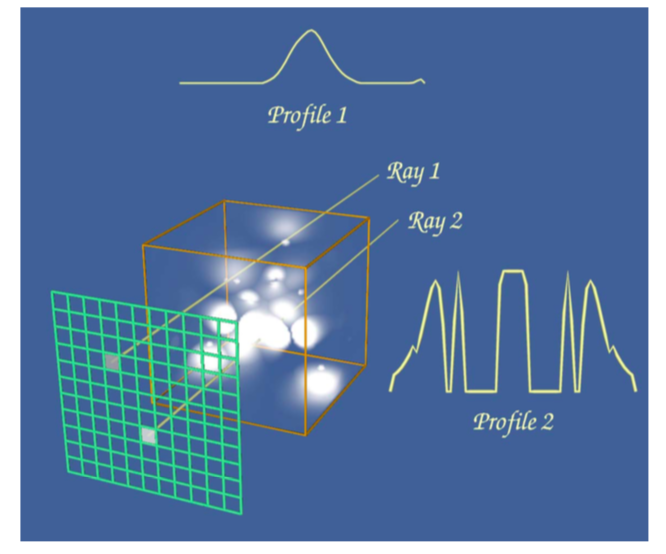
\includegraphics[width=.9\linewidth]{Images/imageorder.png}
  			\caption{Volume rendering Image-Order}
		\end{subfigure}
		\begin{subfigure}{.4\textwidth}
  			\centering
  			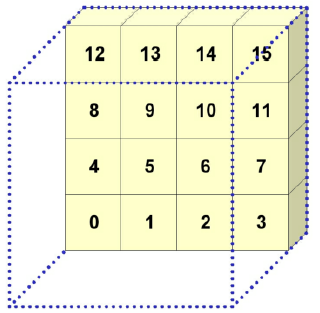
\includegraphics[width=.8\linewidth]{Images/objectorder.png}
  			\caption{Volume rendering Object-Order}
		\end{subfigure}
	\end{figure}	
	
	\begin{multicols}{2}
		Image-Order:
		\begin{itemize}
			\item Noto come ray-tracing;
			\item Itera sui pixel dell'immagine finale.
		\end{itemize}

		\columnbreak

		Object-Order:
		\begin{itemize}
			\item Itera sugli elementi del volume.
		\end{itemize}
	\end{multicols}
	
	\end{frame}
	
	%-----------------------------------------	
	
	\section{Cattura immagini}
	\begin{frame}{Cattura immagini}
	
	\begin{figure}[ht]
    	\centering
    	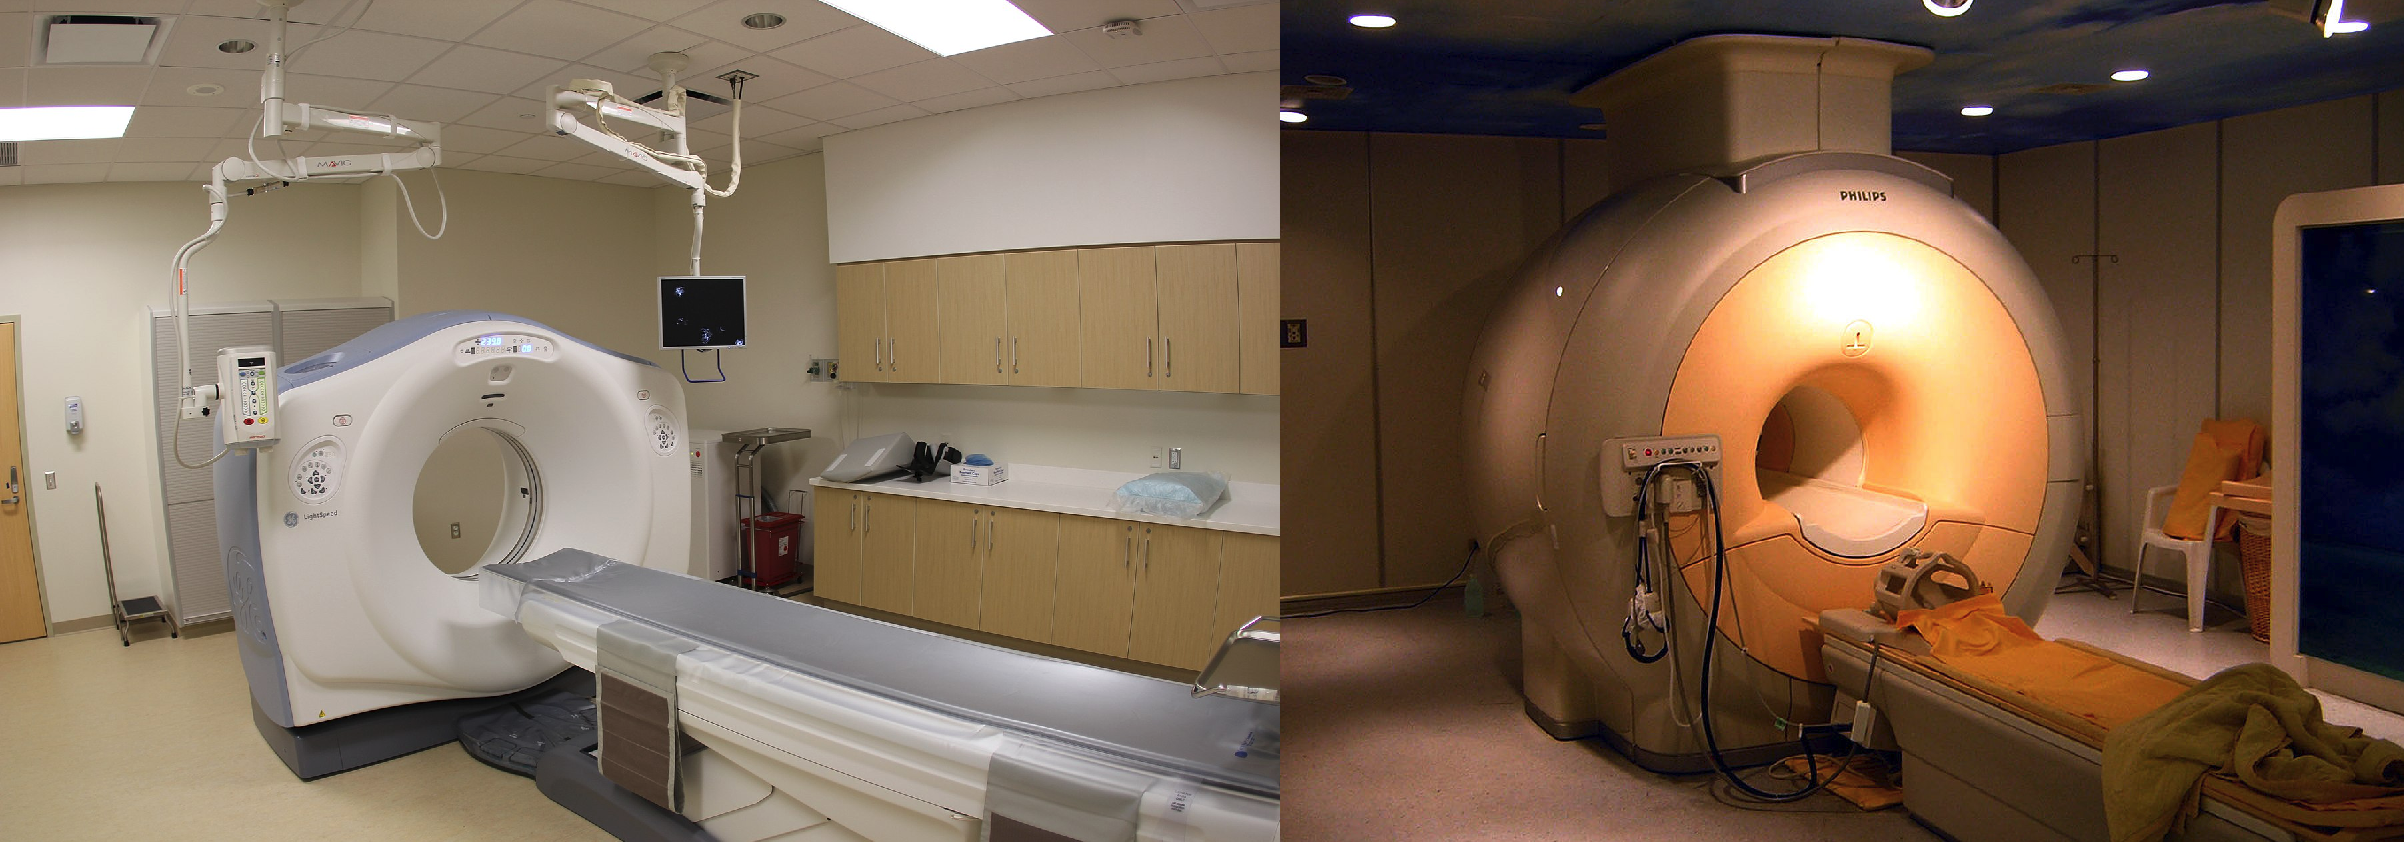
\includegraphics[width=1\textwidth]{Images/medicalscanners.png}
    	\caption{Una macchina per la tomografia computerizzata (TC) a sinistra, e per la risonanza magnetica (RM) a destra.}
	\end{figure}
	
	\end{frame}
	
	%-----------------------------------------	
	
	\section{Ricostruzione immagini}
	\begin{frame}{Ricostruzione immagini (TC)}	
	
	\begin{figure}
		\centering
		\begin{subfigure}{.4\textwidth}
  			\centering
  			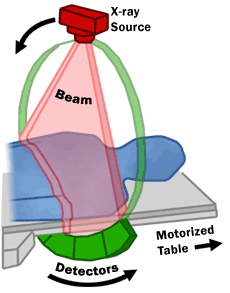
\includegraphics[width=1\linewidth]{Images/CTBeam.png}
		\end{subfigure}
		\begin{subfigure}{.4\textwidth}
  			\centering
  			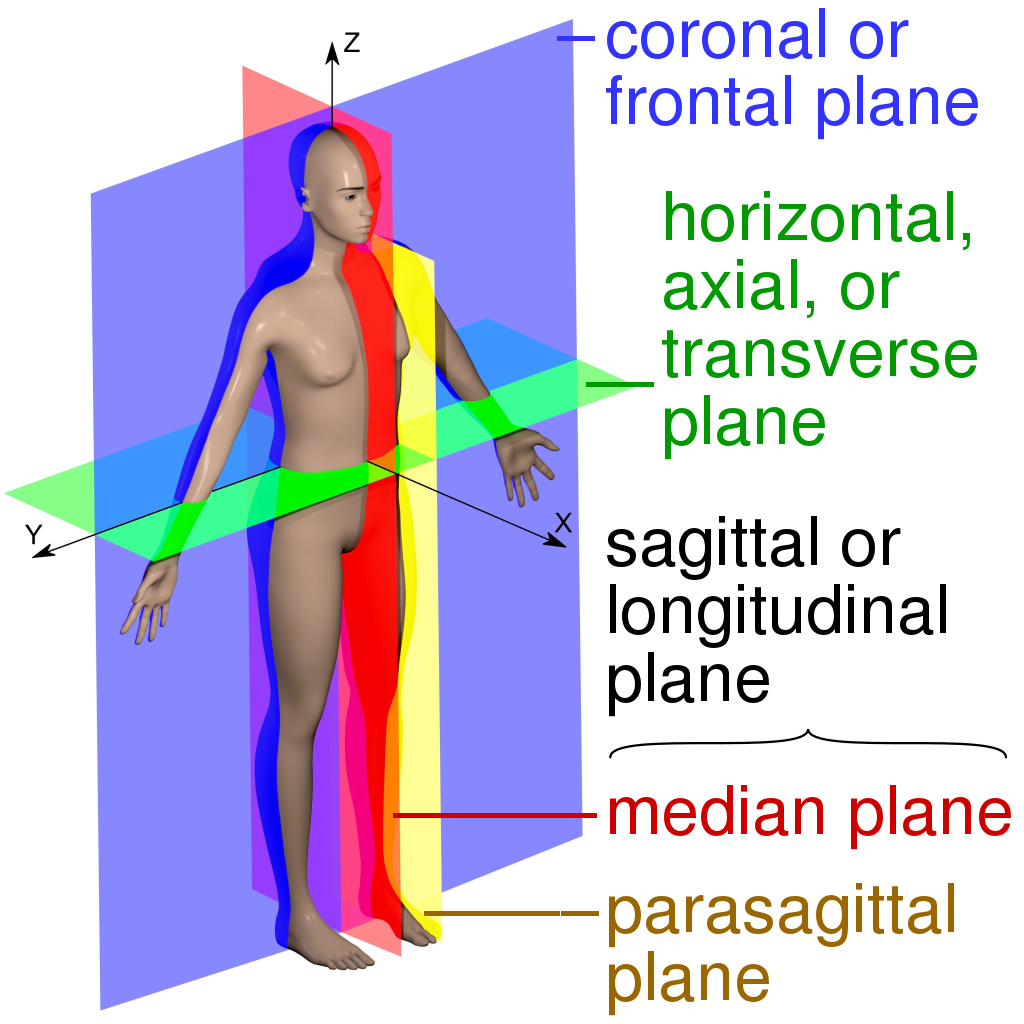
\includegraphics[width=1\linewidth]{Images/anatomyplanes.png}
		\end{subfigure}
	\end{figure}
	
	\end{frame}
	
	%-----------------------------------------	
	
	\section{Struttura file}
	\begin{frame}{Struttura file}
	
	\begin{itemize}
		\item Spesso i file vengono divisi per cartella;
		\item Sono raggruppati a seconda del piano di cattura o di filtri;
		\item Sono conformi allo standard DICOM.
	\end{itemize}
	
	\begin{figure}
		\centering
		\begin{subfigure}{.5\textwidth}
  			\centering
  			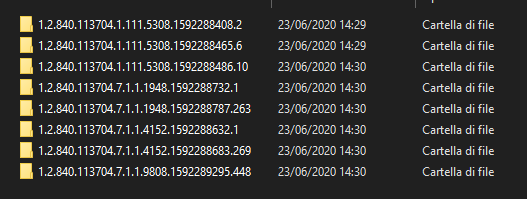
\includegraphics[width=1\linewidth]{Images/ctfolders.png}
		\end{subfigure}
		\begin{subfigure}{.4\textwidth}
  			\centering
  			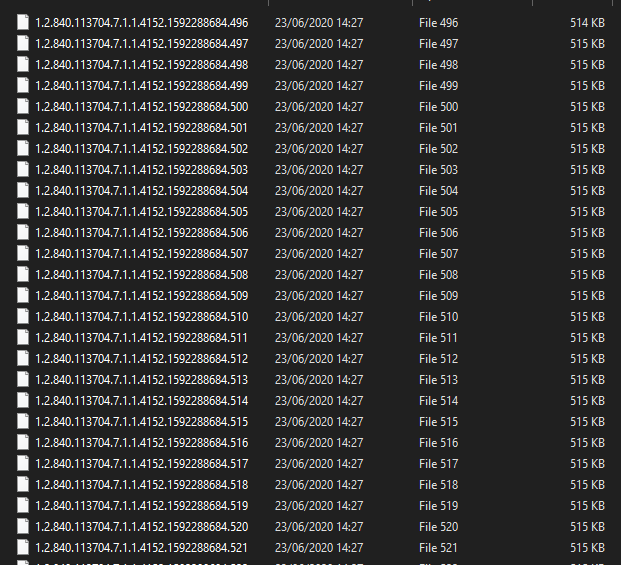
\includegraphics[width=1\linewidth]{Images/ctfiles.png}
		\end{subfigure}
	\end{figure}		
	
	\end{frame}
	
	%-----------------------------------------	
	
	\section{Prima implementazione}
	\begin{frame}{Prima implementazione}
	
	\begin{figure}[ht]
    	\centering
    	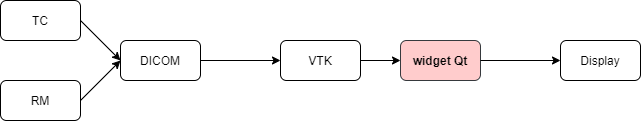
\includegraphics[width=1\textwidth]{Images/primaimplementazione.png}
	\end{figure}
	
	\begin{figure}[ht]
    	\centering
    	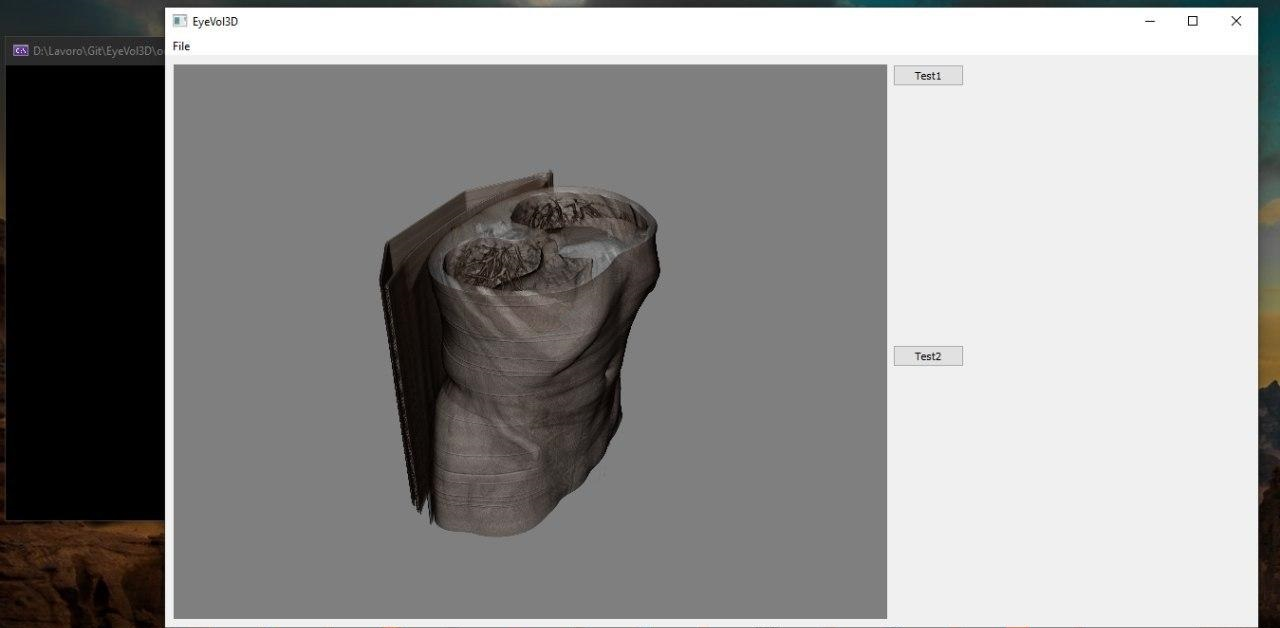
\includegraphics[width=1\textwidth]{Images/firstvolume.jpg}
	\end{figure}	
	
	\end{frame}
	
	%-----------------------------------------	
	
	\section{Aggiunta strumenti}
	\begin{frame}{Aggiunta strumenti}
	
	\begin{figure}[ht]
    	\centering
    	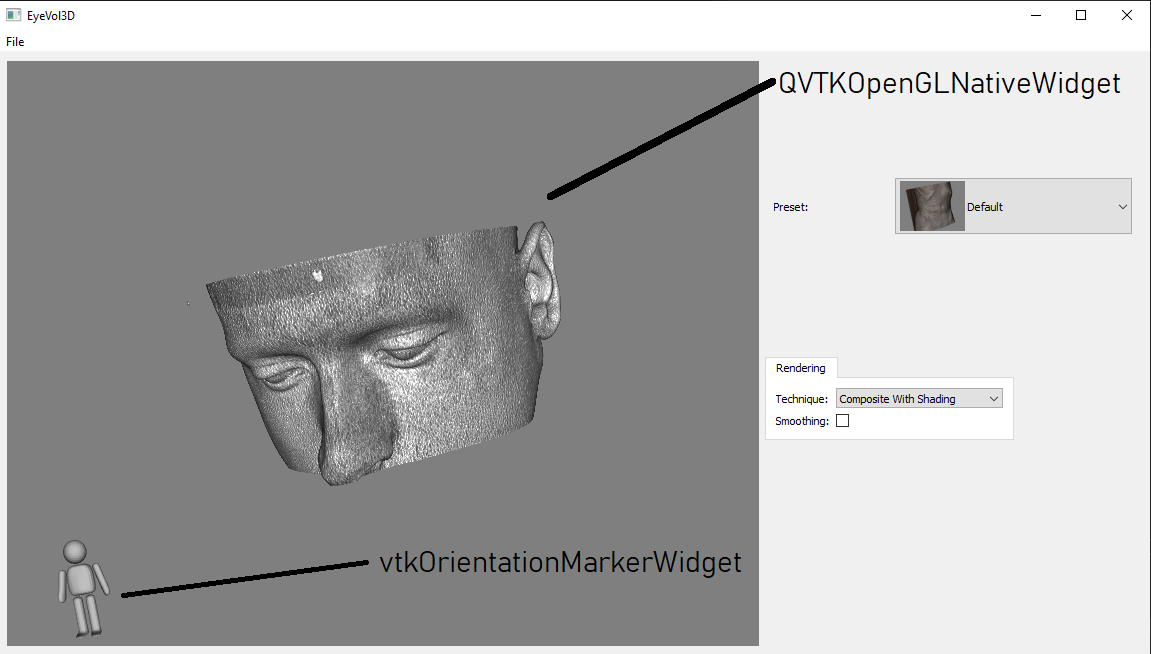
\includegraphics[width=.8\textwidth]{Images/basicwidget.png}
	\end{figure}	
	
	\begin{block}{Altri strumenti non presenti nello screenshot}
		Taglio del volume e editor funzione di Threshold
	\end{block}		
	
	\end{frame}
	
	%-----------------------------------------	
	
	\section{Porting librerie aziendali}
	\begin{frame}{Porting librerie aziendali}

	\begin{itemize}
		\item Portare le librerie aziendali da Qt qmake a CMake;
	\end{itemize}
	
	\begin{figure}[ht]
    	\centering
    	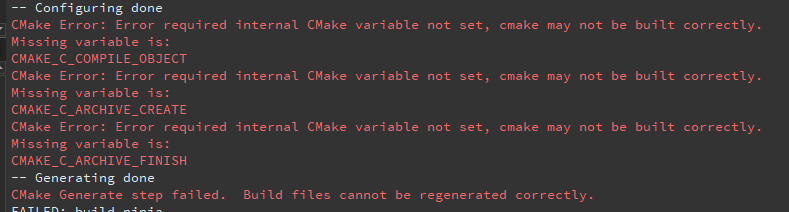
\includegraphics[width=.8\textwidth]{Images/cmakeerror.png}
	\end{figure}
	
	\begin{itemize}
		\item Modificare il software per utilizzarle;
		\item Come copiare le immagini in VTK?
	\end{itemize}
	
	\begin{figure}[ht]
    	\centering
    	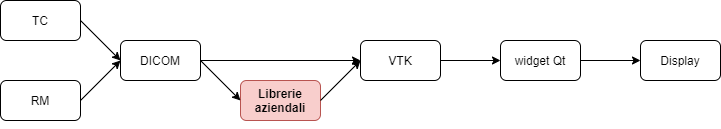
\includegraphics[width=1\textwidth]{Images/librerieaziendali.png}
	\end{figure}
	
	\end{frame}
	
	%-----------------------------------------	
	
	\section{Utilizzo librerie aziendali}
	\begin{frame}{Utilizzo librerie aziendali}
	
	\begin{alertblock}{Difficoltà}
		Copiare le immagini in VTK non è stato intuitivo come previsto
	\end{alertblock}
	
	\begin{figure}[ht]
    	\centering
    	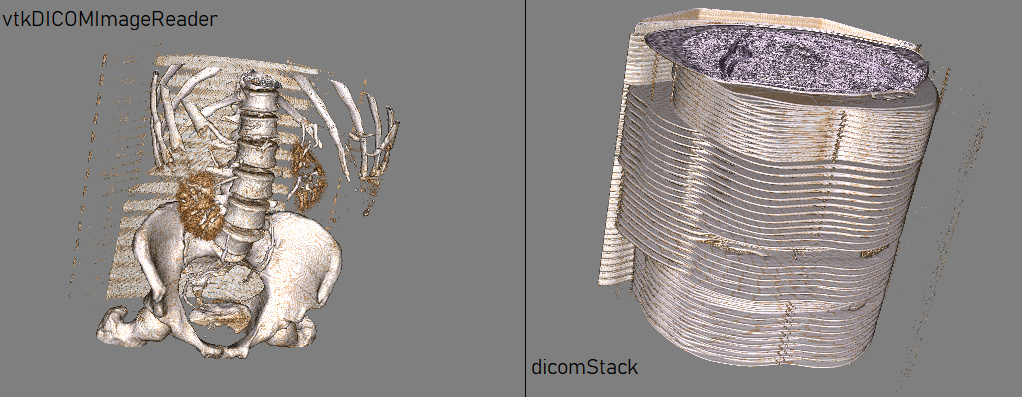
\includegraphics[width=1\textwidth]{Images/volumebrokenorder.jpg}
	\end{figure}
	
	\end{frame}
	
	%-----------------------------------------	
	
	\section{Versione finale TC}
	\begin{frame}{Versione finale}
	
	\begin{figure}[ht]
    	\centering
    	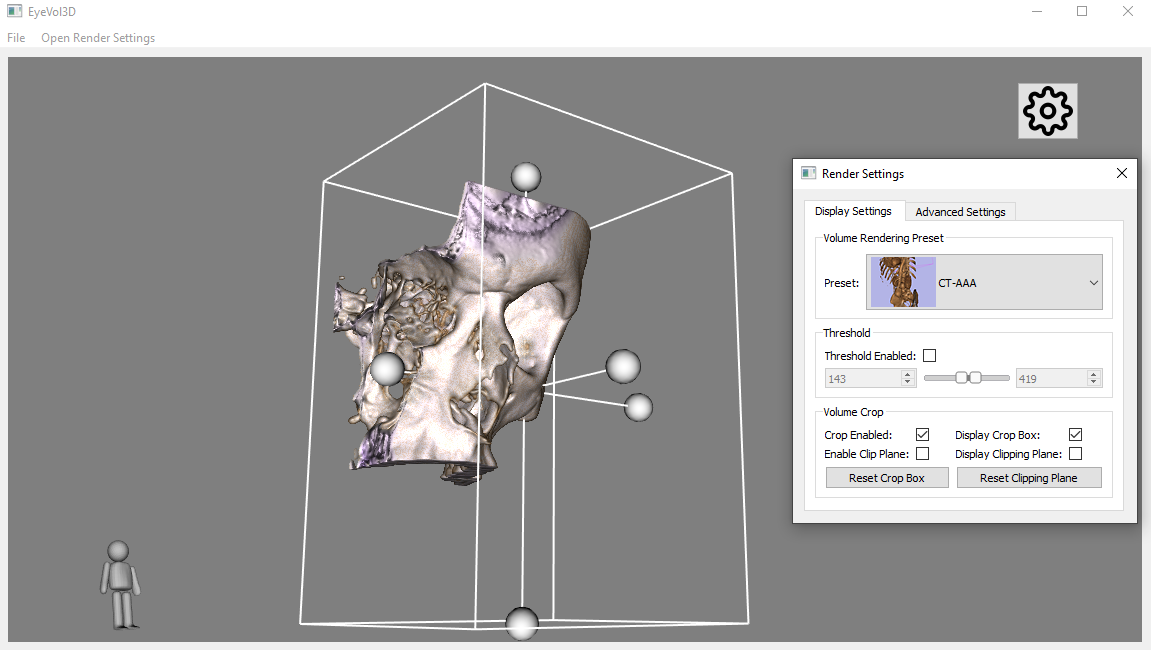
\includegraphics[width=1\textwidth]{Images/finalnewui.png}
	\end{figure}
	
	\end{frame}
	
	%-----------------------------------------	
	
	\section{Versione finale RM}
	\begin{frame}{Versione finale}
	
	\begin{figure}[ht]
    	\centering
    	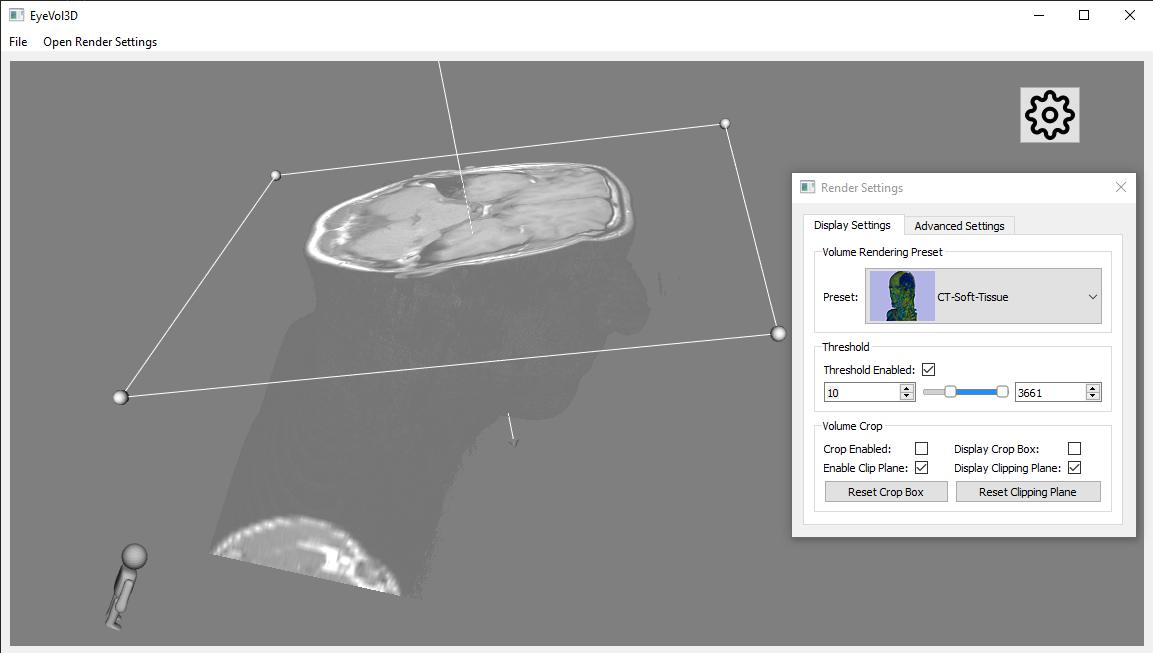
\includegraphics[width=1\textwidth]{Images/rmcapture.png}
	\end{figure}
	
	\end{frame}
	
	%-----------------------------------------	
	
	\section{Testing}
	\begin{frame}{Testing}
	
	\begin{itemize}
		\item Come testare il risultato di un render?
		\item Come fanno altre librerie? Esempio di VTK:
	\end{itemize}	
	
	\begin{figure}[ht]
    	\centering
    	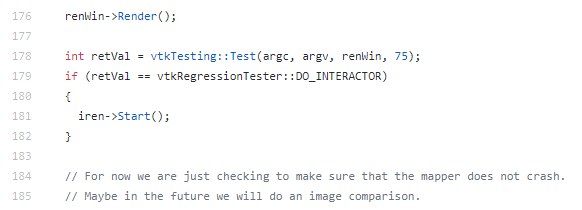
\includegraphics[width=1\textwidth]{Images/vtktests.png}
	\end{figure}
	
	\begin{itemize}
		\item Implementati semplici test di unità
	\end{itemize}
	
	\end{frame}
	
	%-----------------------------------------	
	
	\section{Sviluppi futuri}
	\begin{frame}{Sviluppi futuri}	
	
	\begin{itemize}
		\item Esempio di integrazione del widget in altra applicazione
	\end{itemize}
	
	\begin{figure}[ht]
    	\centering
    	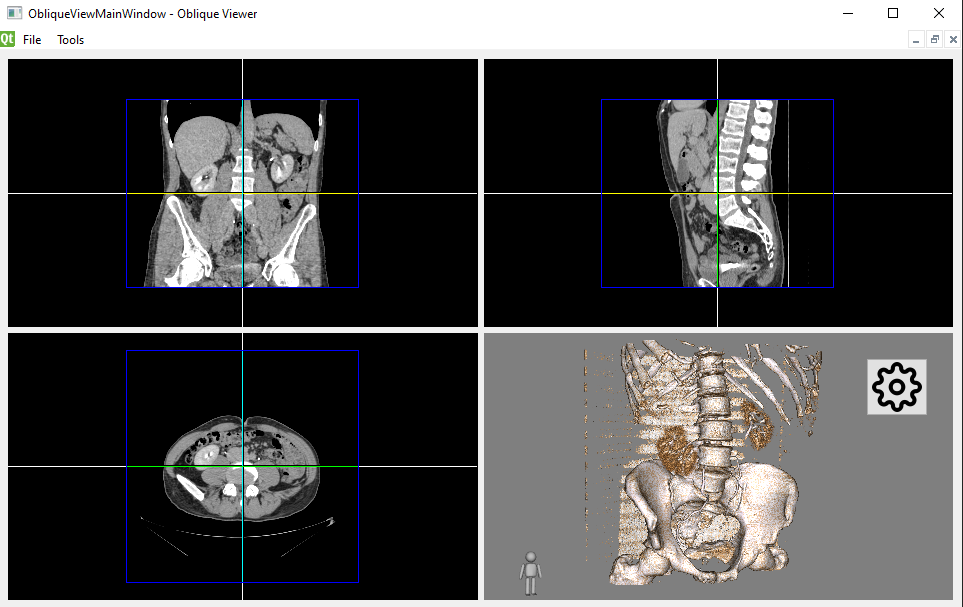
\includegraphics[width=.8\textwidth]{Images/obliqueview.png}
	\end{figure}
	
	\end{frame}
	
	%-----------------------------------------	
	
	\section{Bilancio finale}
	\begin{frame}{Bilancio finale}
	
	Soddisfacimento obiettivi:
	\begin{itemize}
		\item Obiettivi obbligatori 2/2: visualizzatore volumetrico e scelta della funzione di trasferimento;
		\item Obiettivi desiderabili 3/3: impostazione e modifica del taglio del volume, rendering su GPU;
		\item Obiettivi facoltativi 2/3: porting librerie aziendali e studio unit-tests su Qt.
	\end{itemize}
	
	\begin{exampleblock}{Obiettivo non soddisfatto}
	Studio e utilizzo di ITK, considerato solo una possibilità.
	\end{exampleblock}
	
	\end{frame}
	
	%-----------------------------------------	
	
	\section{Note e conclusioni}
	\begin{frame}{Note e conclusioni}
	
	Fonti:
	\begin{itemize}
		\item Foto macchina TC, RM e piani anatomici: \href{https://en.wikipedia.org/wiki/Main_Page}{en.wikipedia.org};
		\item Schema TC: \href{https://www.fda.gov/radiation-emitting-products/medical-x-ray-imaging/what-computed-tomography}{fda.gov};
		\item Tutti i marchi riportati appartengono ai legittimi proprietari.
	\end{itemize}		
	
	\end{frame}
	
	%-----------------------------------------	

\end{document}
